\section{Project Plan}

\begin{minipage}{\linewidth}
  \hspace*{1.7in}
  \begin{rotate}{270}
    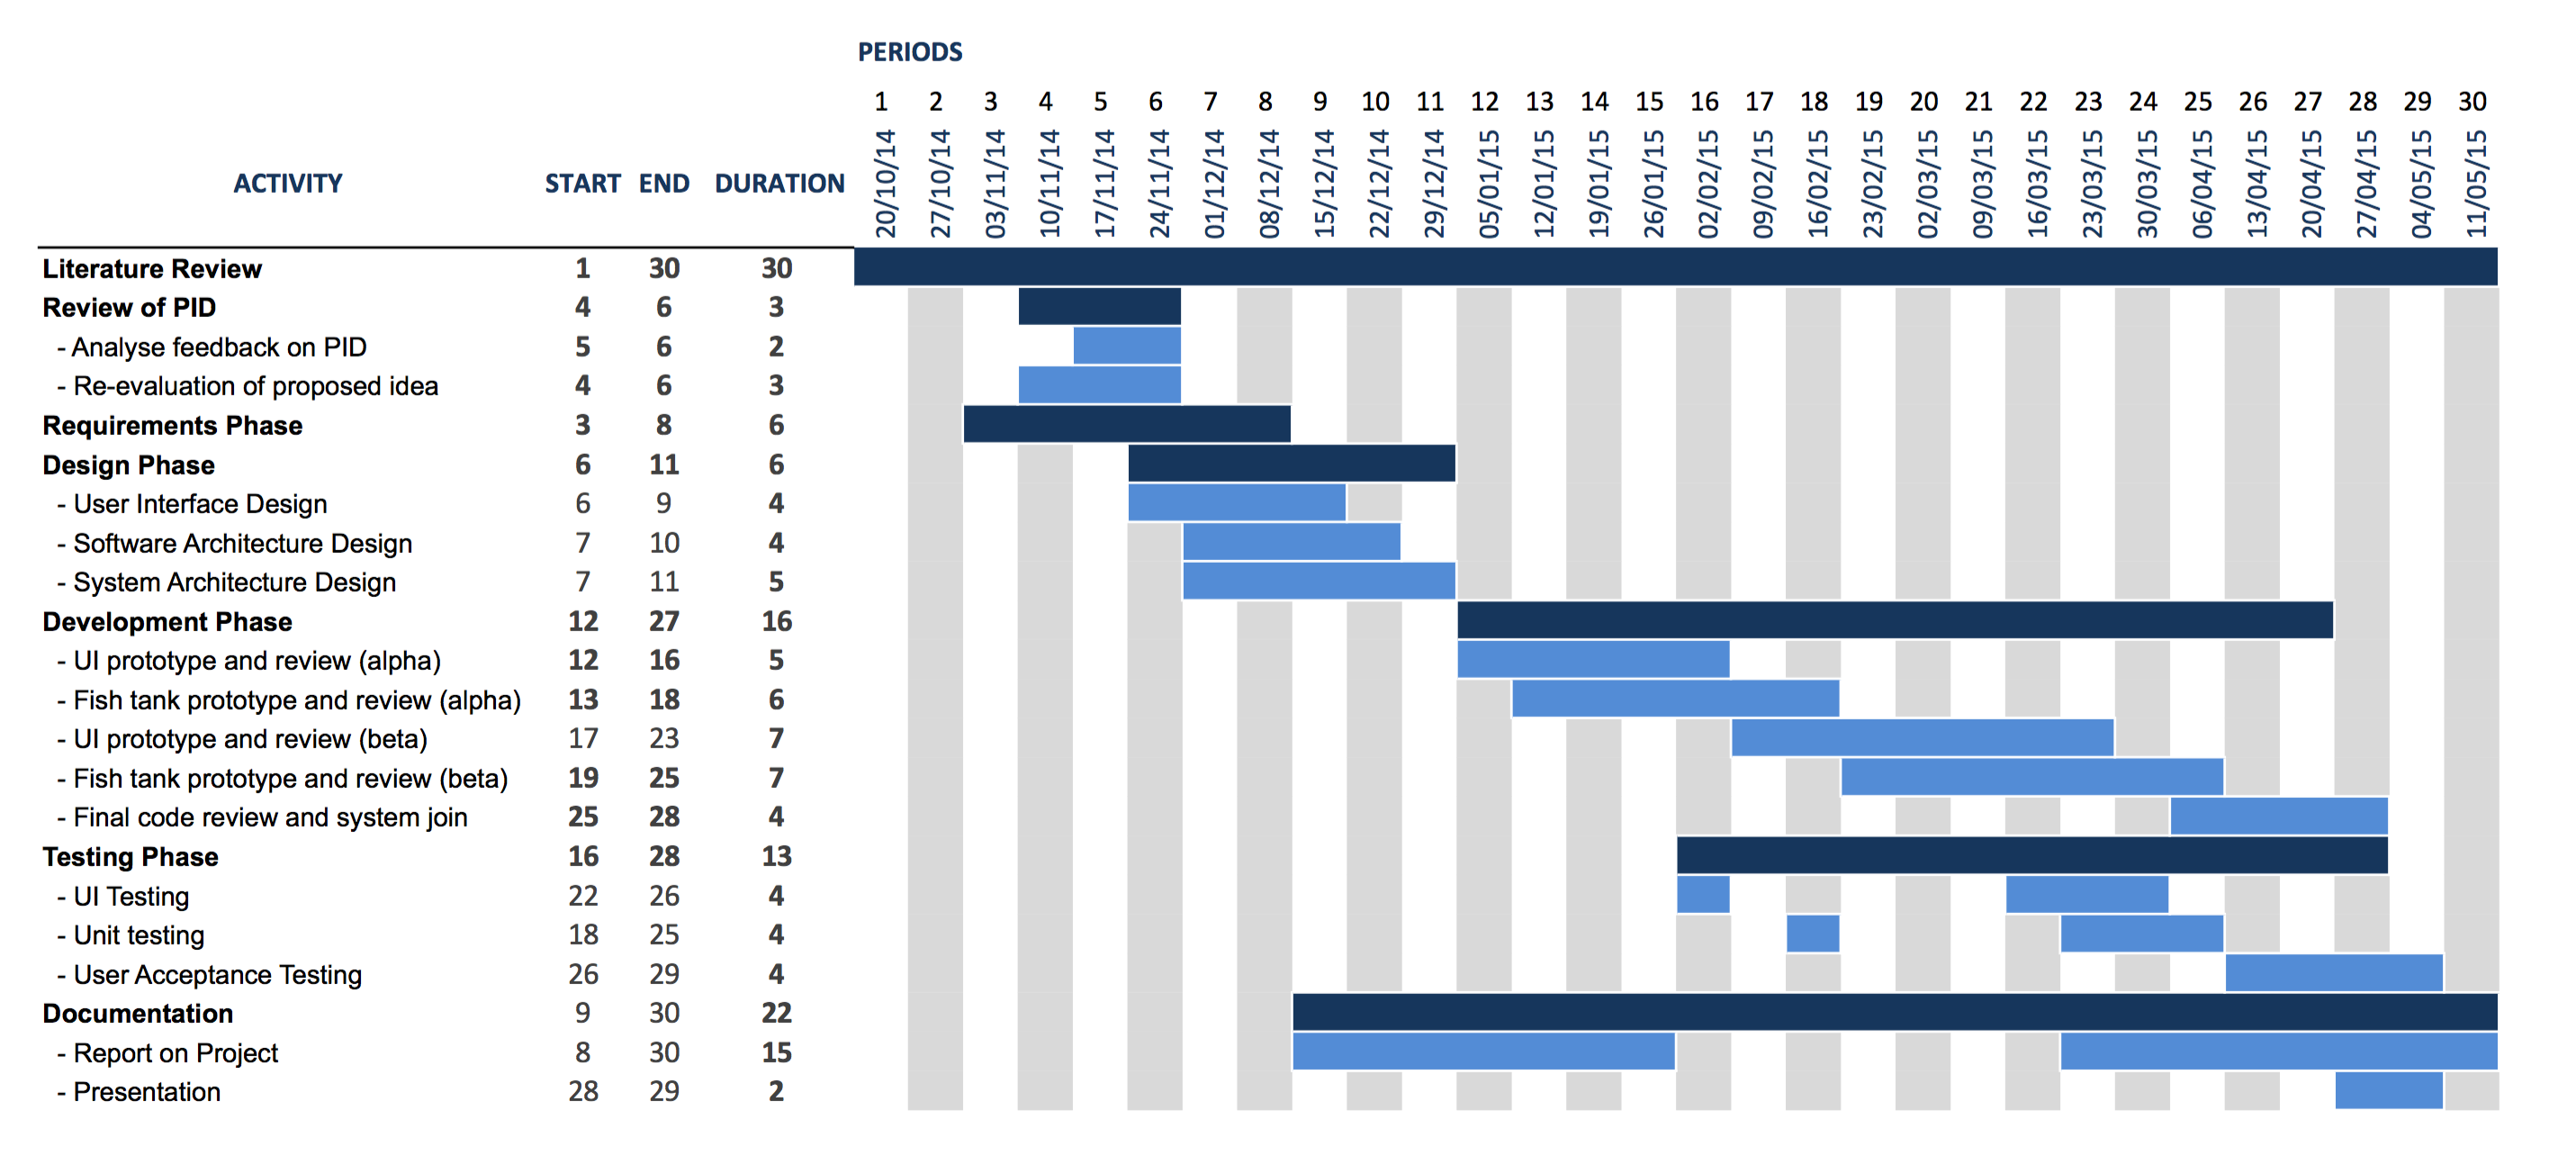
\includegraphics[width=1.28\textwidth]{./img/gantt_chart.png}
    \label{gantt_chart}
  \end{rotate}
\end{minipage}
\clearpage

\subsection{Gantt Chart}
The gantt chart we have provided illustrates how we will aim to complete this project on time.  It includes a break up of all the tasks and the proposed start and finish times.  We will use this gantt chart to track our progress throughout the project and there may be cases whenever we have had to adjust it due to time constrains and other activities outside the project.  

\subsection{Team Roles}
We have tried to arrange the team according to our strengths and weaknesses.  We have tried to consider the different tasks involved in the project and identify the roles that an individual is most likely suited to.  \\
According to Belbin, there are 9 different team roles; three action roles, three people roles and three thought roles.  Our team cover the majority of roles between them; we have shapers, implementers, completes, plants specialists, monitor and team-workers.  Overall this provides us with problems solvers and passionate specialists that have a wealth of knowledge as well as individuals that have a  motivation to complete this task on time and to a high standard. \\
Below, we have defined our roles within the team to best suit our skills and to suit the type of role we are stronger at.

\begin{center}
  \begin{table}[h]
  \begin{tabular}{|l|l|l|}
  \hline
  \multicolumn{1}{|c|}{\textbf{Name}} & \multicolumn{1}{c|}{\textbf{Role}} & \multicolumn{1}{c|}{\textbf{Responsibilities}}                                                                                                                                      \\ \hline
  Jay                                 & Project Secetary, App UI        & \begin{tabular}[c]{@{}l@{}}Organising meetings and following \\* the project timeline.\\ Assisting with development where \\* possible.\end{tabular} \\ \hline
  Oliver                              & Project Manager, Technical Lead                     & \begin{tabular}[c]{@{}l@{}}Leading the technical aspects of the \\* projects forward.\\ Managing cloud infrastructure for \\* both documentation and code.\end{tabular}                     \\ \hline
  Simon                               & Business Development, App UI    & \begin{tabular}[c]{@{}l@{}}Carrying the app forward according \\* to the business model in terms \\* of legal and technological factors.  \\ UI development\end{tabular}                                                              \\ \hline
  \end{tabular}
  \end{table}
\end{center}

\subsection{Project Management}

Responsibilities will be shared throughout the project as there are only three people in the team.  The roles will change throughout the project as it may suit someone else to take on a responsibility at certain stages.  There will also be times when experience will become a factor; we have considered this and tried to align our team roles to match.  During different stages of the project, it may be that we have different activities going on outside of the project that may cause slight readjustments to the gantt chart but this will not effect the overall outcome.  The stronger programmer(s) in the team will have a better understanding of what is involved at the development stage of the project therefore they will be more inclined to take responsibility and delegate tasks.  \\
Every week, we will meet up to discuss any feedback we have based on our previous weeks work and if any decisions need to be taken based on this, these will be made clear and a decision taken before the meeting finishes.  If a decision cannot be taken because of lack of information, we will go away and research the area further and bring the relevant issue(s) up at the next meeting.  We will also use these meetings to determine whether or not we are currently on schedule with the project and to make proactive decisions based upon our current rate of progress.  During each meeting, we will decide what each members tasks for the next week thus allowing us to allocate the right amount of time to complete them.

\subsubsection{Team Communication}
The main communication method for all team members will be through a ``WhatsApp'' group.  All member currently use this as a social messaging service therefore we felt it was a good idea to use this as we always have access to it.  The main idea of this is to send short messages to each other whether it be the whole group or just one individual.  This keeps everyone in the loop.  We can effectively use this to organise meetings and communicate our progress and problems.  We also have gmail accounts that allow us to send communications to our customer (Mike).  \\

Further to this, we all have access to ``Google Drive''.  We have used this to create a folder that each of us have access to.  Here we can post any documents we want the other team members to view and they can instantly access them and make any changes they want; these changes will be globally updated for all users to see.  \\
Initially a ``Trello'' discussion board was used to throw ideas around and discuss potential features of the app as well as a broad business model. \\
We will also be using GitHub.  GitHub is a web based repository that offers Source Code Management (SCM).  SCM is a necessity in a team orientated software development project.  A Version Control System (VCS) allows the developers to make revisions to the code seamlessly and without overwriting someone else changes.  It also allows you to revert to previous versions or examine them where need be; to help identify issues with newer version(s).  This is a very useful tool to have especially when the project involves such a large code base and multiple developers.  

\subsection{Resources}
In order to complete this project, there will be several different resources we will need to have access to.  This can usually be split into three different categories; personnel, funds and non-personnel.  However for this project, the only personnel we have are the three team members and this cannot be expanded on.  Funds is also non-negotiable; standing at £0.  \\
We do have several non-personnel resources - these are resources that we need in order to produce the prototype and documentation.  These are listed below with an explanation as to why these are needed.
\begin{itemize}
\item Raspberry Pi - There is the potential for some software to be developed and put on a hardware device in order to connect with the cloud and stream audio (music).  For prototyping it is likely that pre-existing devices such as the Raspberry Pi will be used. 
\item Speakers - To enable us to listen to the output from the Raspberry Pi
\item Laptops - these enable us to work as a team in any location at any time and for use in the presentation.  
\item Television - to present our idea and prototype at the end of the year.
\end{itemize}
Having the above items will make sure we can complete this project to a good standard and bale us t give a presentation at the end.    

\subsection{Software Development Approach}
Software Development Approaches have existed since the 1970s. They range from rigid, long-term methods such as \emph{Waterfall}. through to experimental and risky approaches like \emph{Extreme Programming}. Factors such as team size, business goals and clients all contribute to choosing the correct approach.\\
To identify the correct software development process to use we must first decide on some attributes of the project of which we can compare across various approaches. The following have been derived from the project ideas and plan:

\begin{enumerate}
  \item \textbf{Team Size} -
    Most of the development throughout this project will be done by one person. This removes the need for large-scale approaches such as \emph{Waterfall} and \emph{Spiral} and instead opens up the possibility of a faster, looser process such as \emph{Agile}.
  \item \textbf{Client Interaction} - 
    If the project idea is accepted we will be allowed to work very closely with a representive from Atos. This means our development approach needs to incorporate this throughout the entire lifecycle, making methodologies such as \emph{Waterfall} less relevant since they do not encourage client interaction during the development stage.
  \item \textbf{Timeline} - 
    The entire development and testing cycle for the project is only a few months, so whatever approach is chosen needs to be dynamic and allow for quick iterations without the need to go through the entire process again. This requirement makes approaches such as \emph{Incremental Development} inappropriate because they add in repeated requirements analysis and architecture design steps that may not be necessary.
  \item \textbf{Deliverable} -
    The client is expecting a working prototype to be delivered at the end of the project. The technology must be built to a satisfactory standard, but does not need to be production-ready nor be immaculately written. This allows for the testing, integration and implementation steps in the software development approach to be removed as a priority and opens up the possibility of using less formal approaches such as \emph{Prototyping} and \emph{Extreme Programming}.
\end{enumerate}
These requirements narrow the scope down to three relevant approaches.  The first one is \textbf{Agile}.  Agile development promotes principles such as continuous improvement, early delivery, adaptive planning and evolutionary development. It breaks tasks down into small increments, with the goal of each increment being a new release. There is a big focus on quick communication and easy feedback, normally achieved by daily standup meetings and regular planning sessions. Whilst the communication principles would be useful for this project, the approach also tends to have a reliance on multiple teams tackling the project which is not relevant.\\
The second approach we could take would be \textbf{Prototyping}.  Software prototyping is perfect for projects where a production-ready deliverable is not required. Each iteration of the project has no requirement to fully work or meet the users' requirements. Instead, the software goes through an iterative modification process until user acceptance is met or the prototype is discarded.  The downfall of prototyping is that it is a very relaxed approach. Client interaction is suggested, not enforced, and often the developers may lose sight of the completed project by getting too involved in a limited prototype which ultimately is only a partial representation of the desired product.\\
Finally, we have \textbf{Rapid Application Development (RAD)}.  RAD is used to describe alternatives to the \emph{Waterfall} approach that focus on iterative development rather than formal, structured planning cycles. The most common definition of RAD, created by James Martin, involves an initial requirements planning stage followed by an iterative construction and user feedback stage.\\

    \begin{minipage}{\linewidth}
      \centering
      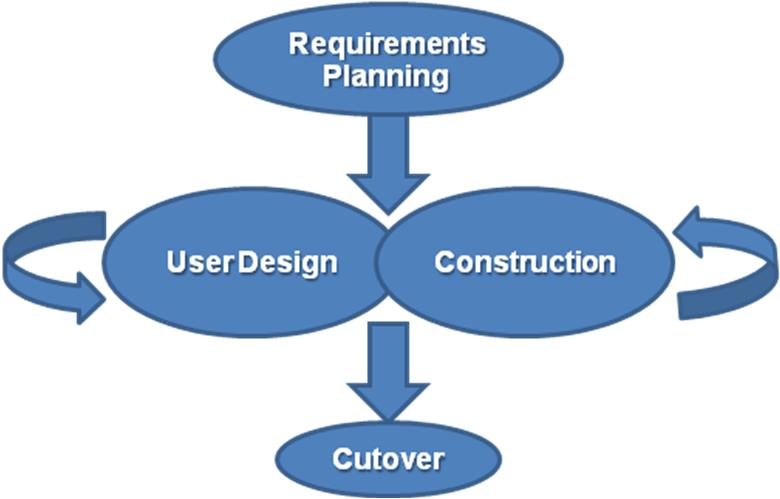
\includegraphics[width=0.5\textwidth]{./img/rad-model.jpg}
      \captionof{figure}{Phases in the James Martin approach to RAD}
    \end{minipage}\\

RAD fits in nicely with the four primary project attributes that we defined above.  RAD has no mandatory definition for team size or interactions.  It requires that development, client feedback and testing go hand in hand.  For this type of project this is ideal.  RAD does not stipulate a restriction on the length of the project thus allowing for the development cycle to be as long as possible before the deadline is reached without the need to stipulate iterations during the planning stages.  Finally, there are no requirements for repetitive testing and quality control.  This can be implemented independently from the software development approach, allowing for testing to be suited to the individual project.\\
The analysis above clearly identifies \textbf{Rapid Application Development} as the most appropriate software development approach for this project.

\subsection{Technical Considerations}
The technical considerations for this project can be divided into two sections: mobile application and server-side systems.

\subsubsection{Mobile Application}
One of the basic top-level requirements for this project is that the end product is centered around a mobile application.  Therefore it is important to ensure that all the technology used or idealised is compatible with as many mobile devices as possible.  If the app starts to have a dependency on niche features, such as NFC and 4G, there is a risk of excluding large quantities of users.\\
For a mobile application, we must consider the platform.  There are currently three major mobile platforms that support apps: Android, iOS and Windows Phone.  Others like Blackberry and Firefox OS either do not have a thriving application community or have a very small user-base.  This project should ideally support all three of the major platforms.  The problem with this is that each one requires applications to be written in different languages.  In order to come to a decision, we need to consider the following:
\begin{itemize}
\item \emph{Native Applications} - A native application is one that is written to work directly with the device's operating system. For example on Android this would mean that the application is written in the programming language Java and that it directly uses the device's native libraries. The advantage this approach is mainly performance, but there are also certain features that are only available for native applications. The disadvantage is that the application has to be written separately for each platform you want to support.
\item \emph{Framework Applications} - To solve the difficulties of supporting multiple platforms, frameworks such as Apache Cordova and Adobe Phonegap have been created. These allow developers to write their applications once and have it automatically work across all major platforms. The downside here is that the application normally exists inside a `wrapper' which can have a negative impact on performance.
\end{itemize}
The \textbf{Technology} behind the mobile device is another area of consideration.  Features such as NFC are starting to become prevalent in many high-end smartphones yet there are still devices that block the use of such technology (such as the iPhone range - the iPhone 6 does have NFC capability but this is only available for apple pay) and there are devices that don't have this capability purely because they are on the lower-end of the market. 

\subsubsection{Server-Side Systems}
Many ideas and concepts in this project revolve around connected data and technology. There are likely to be many different services and systems required in order to complete the project. Designing and architecting will be an important part of ensuring the project is a success.  \\
There are many different styles of \textbf{Software Architecture}. For this project we will be using the \emph{Microservices Architecture}. This is centered around separating out the application into individual services, each one with its own unique responsibility. This fits in nicely with the chosen Software Development Approach - \emph{Rapid Application Development} - since it allows for entire services to be completed in a single development cycle.\\

    \textbf{Advantages}
    \begin{itemize}
      \item Easier debugging
      \item Better fault isolation
      \item Independent service development and deployment
      \item Removes commitment to a specific technolog stack
      \item Avoids monolithic applications and systems
    \end{itemize}

    \textbf{Disadvantages}
    \begin{itemize}
      \item Requires inter-service communication
      \item Testing can be more complicated
      \item Multi-service deployment can be hard to orchestrate
      \item Multiple services means more memory usage
    \end{itemize}
A solid \textbf{Infrastructure} is essential in order to adequately support the numerous software services and systems required for the project. There are several options available when it comes to selecting infrastructure components (servers, database management systems etc):
    \begin{itemize}
      \item \textbf{Cloud Computing} - 
        Cloud-based systems such as \emph{Amazon Web Services} (AWS) and \emph{IBM SoftLayer} allow systems engineers to easily configure and deploy scalable services across the globe. They often support many different types of services (application servers, databases, data processors, queues etc) and can be configured quickly and easily through user interfaces, rather than having to manually set up each service. The downside to cloud-based infrastructure is usually the cost and also the added abstraction; the systems engineer is no longer in direct control of each moving part which can sometimes make fault finding a more laborious process.
      \item \textbf{Dedicated Servers} - 
        Dedicated servers are the more traditional approach to supporting software systems. They give the systems engineer absolute control over the entire infrastructure, however this goes hand-in-hand with the additional responsibility involved in configuring everything by hand. Another concern is redudancy. In a cloud-based system it is very easy to spin up copies of a service in the event of failture, however with a dedicated system you normally need to have servers on standby all the time. Compared to cloud services, dedicated servers can often work out cheaper.
    \end{itemize}
